\documentclass[
  aspectratio=1610, %default screen size (4:3); other values: 1610, 169, 149, 54, 32
% handout,
%  smaller, %uncomment this to fit more text onto the slides (similar to the CD suggestions)
  intlimits %put limits of integrals above and below the integral symbol
]{beamer}

%\usepackage[ngerman]{babel}
%\usepackage[english]{babel}
%\usepackage[UKenglish]{babel}

%my favourite packages
%\usepackage[latin1]{inputenc} %type in accented characters easily, i. e. ä instead of \"a 
%\usepackage{siunitx} %easy input & nice formatting of phys. quantities (number + SI unit)
%\usepackage{latexsym}
%\usepackage{amssymb}
%\usepackage{movie15}
%\usepackage{animate}
%\usepackage{ragged2e}\RaggedRight
\usepackage{ifthen}
\usepackage{mathtools}
\DeclareMathOperator*{\argmin}{arg\,min}

%%%%%%%%%%%%%%%%%%%%%%%%%%%%% some optional settings %%%%%%%%%%%%%%%%%%%%%%%%%%%%%%%%%%%%
%uncomment this if you want the title page text aligned flushleft; CD rules seem to
%demand this, although it looks awful
%\def\titleflushleft{}

%uncomment this if you want frame titles centered
%\def\frametitlecentered{}

%uncomment this if you don't like the wallclock
%do not want clock, does not work with okular
\def\noclock{}

%uncomment this if you don't like the navigation buttons
%\def\nonavigation{}

%uncomment this if you want Arial as the main text font (very ugly),
%no matching math font, using CM-Bright for math text
%\def\arial{}

%uncomment this if you want Helvetica as the main text font (very ugly),
%Helvetica is very similar to Arial; again, no matching math font, using CM-Bright for
%math text
%\def\helvetica{}


\usepackage{helmholtzai}

%%%%%%%%%%%%%%%%%%%%%%%%%%%%%%%%%%%%%%%%%%%%%%%%%%%%%%%%%%%%%%%%%%%%%%%%%%%%%%%%%%%%%%%%%%

\hypersetup{%
  breaklinks,colorlinks,
  %pdfpagemode=FullScreen,
  pdfhighlight=/P,
  linkcolor=hgfdarkblue,
  linkcolor=hgfdarkblue,
  anchorcolor=hgfdarkblue,
  citecolor=hgfdarkblue,
  filecolor=hgfdarkblue,
  menucolor=hgfdarkblue,
  runcolor=hgfdarkblue,
  urlcolor=hgfdarkblue
}

% \usepackage[T1]{fontenc}
% \usepackage[utf8]{inputenc}
% \usepackage{sistyle}
% \usepackage[english]{isodate}
% \usepackage[version=3]{ageschem}
%\usepackage{picins}
% \usepackage{url}
% \usepackage{tabularx}
% \usepackage{multimedia}

%\usepackage{etex}
\usepackage{tikz}
\usetikzlibrary{arrows,decorations.pathmorphing,backgrounds,positioning,fit,petri,calc,shapes.geometric,scopes,fit,spy}
\usepackage{pgfplots}
\pgfplotsset{,compat=1.11}
\tikzset{/pgf/number format/1000 sep={\,}}
%\usepackage[version=3]{mhchem}
\usepackage{calc}
\usepackage[fixed]{fontawesome5}

%\usepackage[export]{adjustbox}

%\usepackage{enotez}
%\def\enmarkstyle{\tiny}

% \usepackage{python}

% \usepackage{dashrule}

%\usepackage{appendixnumberbeamer}

%\input{UserFunkt.tex}
%\SIstyle{USA}

\title{%
 How did we learn
}
\subtitle{DeepLearning540 - Lesson 06 
}
%[short version of authors to be used in footlines]{long version in the title page}
\author{{Peter Steinbach}}

\date{3rd~March~2021}

\institute{%
 \iflanguage{ngerman}{%
  Zentralabteilung Informationsdienste und Computing, Helmholtz-Zentrum Dresden-Rossendorf
 }{%
  Department of Information Services and Computing, Helmholtz-Zentrum Dresden-Rossendorf
 }%
}



%%%%%%%%%%%% document content starts here  %%%%%%%%%%%%%%%%%%%%%%%%%%%
%\AtBeginSubsection

\definecolor{darkgreen}{RGB}{0,130,0}

% \makeatletter
% \let\old@section\section
% \let\section\relax
% \newcommand\section{%
%  \@ifstar\mySectionStar\mySectionNoStar%
% }%
% \newcommand\mySectionNoStar[1]{%
%   \old@section{#1}%
%   \noautobookmark%add excerpt from toc to beginning of section
%   \frame{\frametitle{#1}\tableofcontents[currentsection]}%
%   \autobookmark
% }%
% \newcommand\mySectionStar[1]{%
%   \old@section*{#1}%
% }%
% \makeatother

\renewcommand\footnotesize{\tiny}
\newlength\mytextheight

\newlength\tmplength

\renewcommand\emph{\textbf}

\providecommand{\hidText}[1]{$H_{#1}$}%
\makeatletter
\newcommand{\tikzANN@InputLayerTitle}{Input\\Layer}%
\newcommand{\tikzANN@HiddenLayerTitle}{Hidden\\Layer}%
\newcommand{\tikzANN@OutputLayerTitle}{Output\\Layer}%
\providecommand{\tikzANNInputLayerTitle} {\tikzANN@InputLayerTitle}%
\providecommand{\tikzANNHiddenLayerTitle}{\tikzANN@HiddenLayerTitle}%
\providecommand{\tikzANNOutputLayerTitle}{\tikzANN@OutputLayerTitle}%
\makeatother

\newcommand{\tikzANNResetTitleCommands}{%
\makeatletter
\renewcommand{\tikzANNInputLayerTitle} {\tikzANN@InputLayerTitle}%
\renewcommand{\tikzANNHiddenLayerTitle}{\tikzANN@HiddenLayerTitle}%
\renewcommand{\tikzANNOutputLayerTitle}{\tikzANN@OutputLayerTitle}%
\makeatother
}
\tikzset{synapseNode/.style={}}

\newcommand\tikzANNtpl[2]
{
 \begin{tikzpicture} [
  neuron/.style={circle,minimum size=4em,align=center},
  inNeuron/.style={neuron,draw=blue,fill=blue!20},
  hiddenNeuron/.style={neuron,draw=green,fill=green!20},
  outNeuron/.style={neuron,draw=red,fill=red!20},
  synapseNodeMy/.style={near start,sloped,above,
     outer sep=0ex,inner sep=.2ex, synapseNode},
  every node/.append style={node distance=2em,inner sep=0pt},
  #1
 ]
  \node[inNeuron] (in 0) {\inText{0}};
  \node[inNeuron, below=of in 0] (in 1) {\inText{1}};
  \node[inNeuron, below=of in 1] (in 2) {\inText{2}};

  \node[hiddenNeuron, right=6em of in 0] (hid 0) {\hidText{0}}; 
  \node[hiddenNeuron, right=6em of in 1] (hid 1) {\hidText{1}}; 
  \node[hiddenNeuron, right=6em of in 2] (hid 2) {\hidText{2}}; 

  \node[inner sep=0em,outer sep=0em, fit=(hid 0) (hid 1)] (hidG 01) {};
  \node[inner sep=0em,outer sep=0em, fit=(hid 2) (hid 1)] (hidG 12) {};

  \node[outNeuron, right=6em of hidG 01] (out 0) {\outText{0}}; 
  \node[outNeuron, right=6em of hidG 12] (out 1) {\outText{1}}; 

  \foreach \a in {0,...,2} {
   \foreach \s in {0,...,2} {
    \draw (in \a) -- (hid \s) node[synapseNodeMy] {\synapseIHText{\a}{\s}};
   }}

  \foreach \a in {0,...,2} {
   \foreach \s in {0,...,1} {
    \draw (hid \a) -- (out \s) node[synapseNodeMy] {\synapseHOText{\a}{\s}};
   }}

  \node[above=1.5em of in 0,align=center] {\tikzANNInputLayerTitle};
  \node[above=1.5em of hid 0,align=center] (hidTitle) {\tikzANNHiddenLayerTitle};
  \node[anchor=center,align=center] at (out 0 |- hidTitle) {\tikzANNOutputLayerTitle};

  #2
 \end{tikzpicture}
}

\newcommand\tikzANN[1]{\tikzANNtpl{#1}{}}

\newcommand\tikzANNwBottomIns[2]{\tikzANNtpl{#1}{#2}}

\providecommand{\inText}[1]{$I_{#1}$}%
\providecommand{\hidTextN}[2]{$H^{(#2)}_{#1}$}%
\providecommand{\outText}[1]{$O_{#1}$}%
\providecommand{\synapseIHText}[2]{}%
\providecommand{\synapseHOText}[2]{}%
\providecommand{\synapseHHText}[2]{}%
\newcommand{\tikzMLPResetTextCommands}{%
\renewcommand{\inText}[1]{$I_{##1}$}%
\renewcommand{\hidTextN}[2]{$H_{##1##2}$}%
\renewcommand{\outText}[1]{$O_{##1}$}%
\renewcommand{\synapseIHText}[2]{}%
\renewcommand{\synapseHOText}[2]{}%
}

\makeatletter
\newcommand{\tikzMLP@InputLayerTitle}{Input\\Layer}%
\newcommand{\tikzMLP@HiddenLayerTitle}{Hidden\\Layers}%
\newcommand{\tikzMLP@OutputLayerTitle}{Output\\Layer}%
\providecommand{\tikzMLPInputLayerTitle} {\tikzMLP@InputLayerTitle}%
\providecommand{\tikzMLPHiddenLayerTitle}{\tikzMLP@HiddenLayerTitle}%
\providecommand{\tikzMLPOutputLayerTitle}{\tikzMLP@OutputLayerTitle}%
\makeatother

\newcommand{\tikzMLPResetTitleCommands}{%
\makeatletter
\renewcommand{\tikzMLPInputLayerTitle} {\tikzMLP@InputLayerTitle}%
\renewcommand{\tikzMLPHiddenLayerTitle}{\tikzMLP@HiddenLayerTitle}%
\renewcommand{\tikzMLPOutputLayerTitle}{\tikzMLP@OutputLayerTitle}%
\makeatother
}
\newcommand\tikzMLP[2]
{
 \begin{tikzpicture} [
  neuron/.style={circle,minimum size=2em,align=center},
  inNeuron/.style={neuron,draw=blue,fill=blue!20},
  hiddenNeuron/.style={neuron,draw=green,fill=green!20},
  outNeuron/.style={neuron,draw=red,fill=red!20},
  every node/.append style={node distance=2em,inner sep=0pt},
  #1
 ]
  \node[inNeuron] (in 0) {\inText{0}};
  \node[inNeuron, below=of in 0] (in 1) {\inText{1}};
  \node[inNeuron, below=of in 1] (in 2) {\inText{2}};

  \node[hiddenNeuron, right=of in 0] (hid 0-0) {\hidTextN{0}{0}}; 
  \node[hiddenNeuron, right=of in 1] (hid 1-0) {\hidTextN{1}{0}}; 
  \node[hiddenNeuron, right=of in 2] (hid 2-0) {\hidTextN{2}{0}}; 

  \node[hiddenNeuron, right=of hid 0-0] (hid 0-1) {\hidTextN{0}{1}}; 
  \node[hiddenNeuron, right=of hid 1-0] (hid 1-1) {\hidTextN{1}{1}}; 
  \node[hiddenNeuron, right=of hid 2-0] (hid 2-1) {\hidTextN{2}{1}}; 

  \node[right=1em of hid 0-1] (hiddd 0) {$\ldots$}; 
  \node[right=1em of hid 1-1] (hiddd 1) {$\ldots$}; 
  \node[right=1em of hid 2-1] (hiddd 2) {$\ldots$}; 

  \node[hiddenNeuron, right=1em of hiddd 0] (hid 0-n) {\hidTextN{0}{N}}; 
  \node[hiddenNeuron, right=1em of hiddd 1] (hid 1-n) {\hidTextN{1}{N}}; 
  \node[hiddenNeuron, right=1em of hiddd 2] (hid 2-n) {\hidTextN{2}{N}}; 

  \node[inner sep=0em,outer sep=0em, fit=(hid 0-0) (hid 2-0) (hid 0-n) (hid 2-n)] (hidG) {};
  \node[inner sep=0em,outer sep=0em, fit=(hid 0-n) (hid 1-n)] (hidG 01) {};
  \node[inner sep=0em,outer sep=0em, fit=(hid 2-n) (hid 1-n)] (hidG 12) {};

  \node[outNeuron, right=of hidG 01] (out 0) {\outText{0}}; 
  \node[outNeuron, right=of hidG 12] (out 1) {\outText{1}}; 

  \foreach \a in {0,...,2} {
   \foreach \s in {0,...,2} {
    \draw (in \a) -- (hid \s-0) node[near start,sloped,above,
     outer sep=0ex,inner sep=.2ex] {\synapseIHText{\a}{\s}};
   }}

  \foreach \a in {0,...,2} {
   \foreach \s in {0,...,2} {
    \draw (hid \a-0) -- (hid \s-1) node[near start,sloped,above,
     outer sep=0ex,inner sep=.2ex] {\synapseHHText{\a}{\s}};
   }}

  \foreach \a in {0,...,2} {
   \foreach \s in {0,...,1} {
    \draw (hid \a-n) -- (out \s) node[near start,sloped,above,
     outer sep=0ex,inner sep=.2ex] {\synapseHOText{\a}{\s}};
   }}

  \node[above=1.5em of in 0,align=center] {\tikzMLPInputLayerTitle};
  \node[above=1.5em of hidG,align=center] (hidTitle) {\tikzMLPHiddenLayerTitle};
  \node[anchor=center,align=center] at (out 0 |- hidTitle) {\tikzMLPOutputLayerTitle};

  #2
 \end{tikzpicture}
}


\renewcommand{\arraystretch}{1.2}

% required for pygment syntax-highlighting
\usepackage{fancyvrb}

\makeatletter
\def\PY@reset{\let\PY@it=\relax \let\PY@bf=\relax%
    \let\PY@ul=\relax \let\PY@tc=\relax%
    \let\PY@bc=\relax \let\PY@ff=\relax}
\def\PY@tok#1{\csname PY@tok@#1\endcsname}
\def\PY@toks#1+{\ifx\relax#1\empty\else%
    \PY@tok{#1}\expandafter\PY@toks\fi}
\def\PY@do#1{\PY@bc{\PY@tc{\PY@ul{%
    \PY@it{\PY@bf{\PY@ff{#1}}}}}}}
\def\PY#1#2{\PY@reset\PY@toks#1+\relax+\PY@do{#2}}

\expandafter\def\csname PY@tok@w\endcsname{\def\PY@tc##1{\textcolor[rgb]{0.73,0.73,0.73}{##1}}}
\expandafter\def\csname PY@tok@c\endcsname{\let\PY@it=\textit\def\PY@tc##1{\textcolor[rgb]{0.38,0.63,0.69}{##1}}}
\expandafter\def\csname PY@tok@cp\endcsname{\def\PY@tc##1{\textcolor[rgb]{0.00,0.44,0.13}{##1}}}
\expandafter\def\csname PY@tok@cs\endcsname{\def\PY@tc##1{\textcolor[rgb]{0.38,0.63,0.69}{##1}}\def\PY@bc##1{\setlength{\fboxsep}{0pt}\colorbox[rgb]{1.00,0.94,0.94}{\strut ##1}}}
\expandafter\def\csname PY@tok@k\endcsname{\let\PY@bf=\textbf\def\PY@tc##1{\textcolor[rgb]{0.00,0.44,0.13}{##1}}}
\expandafter\def\csname PY@tok@kp\endcsname{\def\PY@tc##1{\textcolor[rgb]{0.00,0.44,0.13}{##1}}}
\expandafter\def\csname PY@tok@kt\endcsname{\def\PY@tc##1{\textcolor[rgb]{0.56,0.13,0.00}{##1}}}
\expandafter\def\csname PY@tok@o\endcsname{\def\PY@tc##1{\textcolor[rgb]{0.40,0.40,0.40}{##1}}}
\expandafter\def\csname PY@tok@ow\endcsname{\let\PY@bf=\textbf\def\PY@tc##1{\textcolor[rgb]{0.00,0.44,0.13}{##1}}}
\expandafter\def\csname PY@tok@nb\endcsname{\def\PY@tc##1{\textcolor[rgb]{0.00,0.44,0.13}{##1}}}
\expandafter\def\csname PY@tok@nf\endcsname{\def\PY@tc##1{\textcolor[rgb]{0.02,0.16,0.49}{##1}}}
\expandafter\def\csname PY@tok@nc\endcsname{\let\PY@bf=\textbf\def\PY@tc##1{\textcolor[rgb]{0.05,0.52,0.71}{##1}}}
\expandafter\def\csname PY@tok@nn\endcsname{\let\PY@bf=\textbf\def\PY@tc##1{\textcolor[rgb]{0.05,0.52,0.71}{##1}}}
\expandafter\def\csname PY@tok@ne\endcsname{\def\PY@tc##1{\textcolor[rgb]{0.00,0.44,0.13}{##1}}}
\expandafter\def\csname PY@tok@nv\endcsname{\def\PY@tc##1{\textcolor[rgb]{0.73,0.38,0.84}{##1}}}
\expandafter\def\csname PY@tok@no\endcsname{\def\PY@tc##1{\textcolor[rgb]{0.38,0.68,0.84}{##1}}}
\expandafter\def\csname PY@tok@nl\endcsname{\let\PY@bf=\textbf\def\PY@tc##1{\textcolor[rgb]{0.00,0.13,0.44}{##1}}}
\expandafter\def\csname PY@tok@ni\endcsname{\let\PY@bf=\textbf\def\PY@tc##1{\textcolor[rgb]{0.84,0.33,0.22}{##1}}}
\expandafter\def\csname PY@tok@na\endcsname{\def\PY@tc##1{\textcolor[rgb]{0.25,0.44,0.63}{##1}}}
\expandafter\def\csname PY@tok@nt\endcsname{\let\PY@bf=\textbf\def\PY@tc##1{\textcolor[rgb]{0.02,0.16,0.45}{##1}}}
\expandafter\def\csname PY@tok@nd\endcsname{\let\PY@bf=\textbf\def\PY@tc##1{\textcolor[rgb]{0.33,0.33,0.33}{##1}}}
\expandafter\def\csname PY@tok@s\endcsname{\def\PY@tc##1{\textcolor[rgb]{0.25,0.44,0.63}{##1}}}
\expandafter\def\csname PY@tok@sd\endcsname{\let\PY@it=\textit\def\PY@tc##1{\textcolor[rgb]{0.25,0.44,0.63}{##1}}}
\expandafter\def\csname PY@tok@si\endcsname{\let\PY@it=\textit\def\PY@tc##1{\textcolor[rgb]{0.44,0.63,0.82}{##1}}}
\expandafter\def\csname PY@tok@se\endcsname{\let\PY@bf=\textbf\def\PY@tc##1{\textcolor[rgb]{0.25,0.44,0.63}{##1}}}
\expandafter\def\csname PY@tok@sr\endcsname{\def\PY@tc##1{\textcolor[rgb]{0.14,0.33,0.53}{##1}}}
\expandafter\def\csname PY@tok@ss\endcsname{\def\PY@tc##1{\textcolor[rgb]{0.32,0.47,0.09}{##1}}}
\expandafter\def\csname PY@tok@sx\endcsname{\def\PY@tc##1{\textcolor[rgb]{0.78,0.36,0.04}{##1}}}
\expandafter\def\csname PY@tok@m\endcsname{\def\PY@tc##1{\textcolor[rgb]{0.25,0.63,0.44}{##1}}}
\expandafter\def\csname PY@tok@gh\endcsname{\let\PY@bf=\textbf\def\PY@tc##1{\textcolor[rgb]{0.00,0.00,0.50}{##1}}}
\expandafter\def\csname PY@tok@gu\endcsname{\let\PY@bf=\textbf\def\PY@tc##1{\textcolor[rgb]{0.50,0.00,0.50}{##1}}}
\expandafter\def\csname PY@tok@gd\endcsname{\def\PY@tc##1{\textcolor[rgb]{0.63,0.00,0.00}{##1}}}
\expandafter\def\csname PY@tok@gi\endcsname{\def\PY@tc##1{\textcolor[rgb]{0.00,0.63,0.00}{##1}}}
\expandafter\def\csname PY@tok@gr\endcsname{\def\PY@tc##1{\textcolor[rgb]{1.00,0.00,0.00}{##1}}}
\expandafter\def\csname PY@tok@ge\endcsname{\let\PY@it=\textit}
\expandafter\def\csname PY@tok@gs\endcsname{\let\PY@bf=\textbf}
\expandafter\def\csname PY@tok@gp\endcsname{\let\PY@bf=\textbf\def\PY@tc##1{\textcolor[rgb]{0.78,0.36,0.04}{##1}}}
\expandafter\def\csname PY@tok@go\endcsname{\def\PY@tc##1{\textcolor[rgb]{0.53,0.53,0.53}{##1}}}
\expandafter\def\csname PY@tok@gt\endcsname{\def\PY@tc##1{\textcolor[rgb]{0.00,0.27,0.87}{##1}}}
\expandafter\def\csname PY@tok@err\endcsname{\def\PY@bc##1{\setlength{\fboxsep}{0pt}\fcolorbox[rgb]{1.00,0.00,0.00}{1,1,1}{\strut ##1}}}
\expandafter\def\csname PY@tok@kc\endcsname{\let\PY@bf=\textbf\def\PY@tc##1{\textcolor[rgb]{0.00,0.44,0.13}{##1}}}
\expandafter\def\csname PY@tok@kd\endcsname{\let\PY@bf=\textbf\def\PY@tc##1{\textcolor[rgb]{0.00,0.44,0.13}{##1}}}
\expandafter\def\csname PY@tok@kn\endcsname{\let\PY@bf=\textbf\def\PY@tc##1{\textcolor[rgb]{0.00,0.44,0.13}{##1}}}
\expandafter\def\csname PY@tok@kr\endcsname{\let\PY@bf=\textbf\def\PY@tc##1{\textcolor[rgb]{0.00,0.44,0.13}{##1}}}
\expandafter\def\csname PY@tok@bp\endcsname{\def\PY@tc##1{\textcolor[rgb]{0.00,0.44,0.13}{##1}}}
\expandafter\def\csname PY@tok@fm\endcsname{\def\PY@tc##1{\textcolor[rgb]{0.02,0.16,0.49}{##1}}}
\expandafter\def\csname PY@tok@vc\endcsname{\def\PY@tc##1{\textcolor[rgb]{0.73,0.38,0.84}{##1}}}
\expandafter\def\csname PY@tok@vg\endcsname{\def\PY@tc##1{\textcolor[rgb]{0.73,0.38,0.84}{##1}}}
\expandafter\def\csname PY@tok@vi\endcsname{\def\PY@tc##1{\textcolor[rgb]{0.73,0.38,0.84}{##1}}}
\expandafter\def\csname PY@tok@vm\endcsname{\def\PY@tc##1{\textcolor[rgb]{0.73,0.38,0.84}{##1}}}
\expandafter\def\csname PY@tok@sa\endcsname{\def\PY@tc##1{\textcolor[rgb]{0.25,0.44,0.63}{##1}}}
\expandafter\def\csname PY@tok@sb\endcsname{\def\PY@tc##1{\textcolor[rgb]{0.25,0.44,0.63}{##1}}}
\expandafter\def\csname PY@tok@sc\endcsname{\def\PY@tc##1{\textcolor[rgb]{0.25,0.44,0.63}{##1}}}
\expandafter\def\csname PY@tok@dl\endcsname{\def\PY@tc##1{\textcolor[rgb]{0.25,0.44,0.63}{##1}}}
\expandafter\def\csname PY@tok@s2\endcsname{\def\PY@tc##1{\textcolor[rgb]{0.25,0.44,0.63}{##1}}}
\expandafter\def\csname PY@tok@sh\endcsname{\def\PY@tc##1{\textcolor[rgb]{0.25,0.44,0.63}{##1}}}
\expandafter\def\csname PY@tok@s1\endcsname{\def\PY@tc##1{\textcolor[rgb]{0.25,0.44,0.63}{##1}}}
\expandafter\def\csname PY@tok@mb\endcsname{\def\PY@tc##1{\textcolor[rgb]{0.25,0.63,0.44}{##1}}}
\expandafter\def\csname PY@tok@mf\endcsname{\def\PY@tc##1{\textcolor[rgb]{0.25,0.63,0.44}{##1}}}
\expandafter\def\csname PY@tok@mh\endcsname{\def\PY@tc##1{\textcolor[rgb]{0.25,0.63,0.44}{##1}}}
\expandafter\def\csname PY@tok@mi\endcsname{\def\PY@tc##1{\textcolor[rgb]{0.25,0.63,0.44}{##1}}}
\expandafter\def\csname PY@tok@il\endcsname{\def\PY@tc##1{\textcolor[rgb]{0.25,0.63,0.44}{##1}}}
\expandafter\def\csname PY@tok@mo\endcsname{\def\PY@tc##1{\textcolor[rgb]{0.25,0.63,0.44}{##1}}}
\expandafter\def\csname PY@tok@ch\endcsname{\let\PY@it=\textit\def\PY@tc##1{\textcolor[rgb]{0.38,0.63,0.69}{##1}}}
\expandafter\def\csname PY@tok@cm\endcsname{\let\PY@it=\textit\def\PY@tc##1{\textcolor[rgb]{0.38,0.63,0.69}{##1}}}
\expandafter\def\csname PY@tok@cpf\endcsname{\let\PY@it=\textit\def\PY@tc##1{\textcolor[rgb]{0.38,0.63,0.69}{##1}}}
\expandafter\def\csname PY@tok@c1\endcsname{\let\PY@it=\textit\def\PY@tc##1{\textcolor[rgb]{0.38,0.63,0.69}{##1}}}

\def\PYZbs{\char`\\}
\def\PYZus{\char`\_}
\def\PYZob{\char`\{}
\def\PYZcb{\char`\}}
\def\PYZca{\char`\^}
\def\PYZam{\char`\&}
\def\PYZlt{\char`\<}
\def\PYZgt{\char`\>}
\def\PYZsh{\char`\#}
\def\PYZpc{\char`\%}
\def\PYZdl{\char`\$}
\def\PYZhy{\char`\-}
\def\PYZsq{\char`\'}
\def\PYZdq{\char`\"}
\def\PYZti{\char`\~}
% for compatibility with earlier versions
\def\PYZat{@}
\def\PYZlb{[}
\def\PYZrb{]}
\makeatother



%%%%%%%%%%%%%%%%%%%%%%%%%%%%%%%%%%%%%%%%%%%%%%%%%%%%%%%%%%%%%%%%%%%%%%%%%%%%%%%%
% 

\begin{document}
 
\maketitle

\begin{frame}
 \frametitle{Recap: Fitting the Penguin Dataset}


 \begin{block}{inputs}
   \begin{itemize}
   \item 3 features \newline
     (\texttt{flipper\_length\_mm}, \texttt{bill\_depth\_mm}, \texttt{bill\_length\_mm})
   \item 3 inputs means $\vec{x} \in \mathbb{R}^{3}$
   \end{itemize}
 \end{block}

 \begin{block}{outputs}
   \begin{itemize}
   \item probability for being of \texttt{Adelie} or \texttt{not Adelie} 
   \item using one-hot-encoding
   \item 2 outputs means  $\vec{y} \in \mathbb{R}^{2}$
   \end{itemize}
 \end{block}

 
 \begin{alertblock}{Note}
 \centering
   \textbf{classification with supervised learning!}
 \end{alertblock}
   

\end{frame}


\begin{frame}
 \frametitle{Code that needs (some) explanation}

 \begin{Verbatim}[commandchars=\\\{\},numbers=left,firstnumber=1,stepnumber=1,xleftmargin=.5em,numbersep=1em]
\PY{c+c1}{\PYZsh{} create model}
\PY{n}{model}\PY{o}{.}\PY{n}{compile}\PY{p}{(}\PY{n}{loss}\PY{o}{=}\PY{l+s+s1}{\PYZsq{}}\PY{l+s+s1}{categorical\PYZus{}crossentropy}\PY{l+s+s1}{\PYZsq{}}\PY{p}{,}
              \PY{n}{optimizer}\PY{o}{=}\PY{l+s+s1}{\PYZsq{}}\PY{l+s+s1}{sgd}\PY{l+s+s1}{\PYZsq{}}\PY{p}{,}
              \PY{n}{metrics}\PY{o}{=}\PY{p}{[}\PY{l+s+s1}{\PYZsq{}}\PY{l+s+s1}{accuracy}\PY{l+s+s1}{\PYZsq{}}\PY{p}{]}\PY{p}{)}
\end{Verbatim}

 
\end{frame}

\begin{frame}
  \frametitle{supervised learning in one slide\footnote{credits to Uwe Schmidt}}
  \vfill
  \begin{exampleblock}{}
   \begin{itemize}
   \item given $m$ input pairs in a dataset $\mathcal{D} = \{\langle \vec{x}_i, y_i\rangle \dots \}$ with $x \in \mathbb{R}^n$, $y \in \mathbb{R}$
   \item we would like to train a model $f$ with parameters $\vartheta$ such that 
     \begin{equation*}
     \vec{y} = f(\vec{x}, \vartheta)
   \end{equation*}
   \item we optimize a loss function $\mathcal{L}$ in such a fashion that 
     \begin{equation*}
     \vartheta \approx \argmin_{\vartheta} \mathcal{L}( \vec{y}^{\,true}, f(\vec{x}, \vartheta) )
   \end{equation*}
   \item during optimisation with gradient descent, parameters $\vartheta$ at step $s$ are given by
     
     \begin{equation*}
\vartheta_{s+1} = \vartheta_{s} + \eta \nabla_{\vartheta}L( \vec{y}^{\,true}, f(\vec{x}, \vartheta_{s}))
\end{equation*}

   \end{itemize}
 \end{exampleblock}
  \vfill
  
\end{frame}


 \begin{frame}
 \frametitle{Weight Update Rule}

 \begin{equation*}
\vartheta_{s+1} = \vartheta_{s} + \eta \nabla_{\vartheta}L( \vec{y}^{\,true}, f(\vec{x}, \vartheta_{s}))
\end{equation*}

\begin{exampleblock}{gradient descent}
  \begin{center}
    free parameter $\eta$ known as the learning rate
  \end{center}
\end{exampleblock}

\begin{columns}
  \begin{column}{.45\textwidth}
    \begin{alertblock}{Classic Gradient Descent}
    \begin{itemize}
    \item using the full training set
    \item problem: does not scale with size of dataset
    \end{itemize}
  \end{alertblock}
\end{column}

\begin{column}{.45\textwidth}
  
  \begin{alertblock}{``Online'' Gradient Descent}
    \begin{itemize}
    \item using the one datum at a time
    \item problem: expensive to compute, strongly depends on $eta$
    \end{itemize}
  \end{alertblock}
    
  \end{column}
\end{columns}

\end{frame}

 \begin{frame}
   \frametitle{Stochastic gradient descent}
   
\begin{columns}
  \begin{column}{.45\textwidth}
    
    \begin{block}{mini-batch based stochastic gradient descent}

      \begin{equation*}
\vartheta_{s+1} = \vartheta_{s} + \eta \nabla_{\vartheta}L( \vec{y}^{\,true}, f(\vec{x}, \vartheta_{s}))
\end{equation*}

\begin{itemize}
\item randomly split training set in mini batches, e.g. $b=32$
\item completing one batch is referred to as a \texttt{step}
\item completing the entire dataset is referred to as an \texttt{epoch}
\end{itemize}
\end{block}
\end{column}

\begin{column}{.45\textwidth}
  \footnotesize
  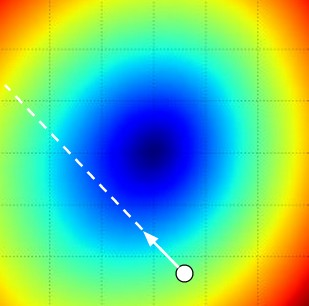
\includegraphics[width=\textwidth]{figures/stepsize}\\
  from \href{https://cs231n.github.io/optimization-1/}{Stanford CS231n}
  \end{column}
\end{columns}


\end{frame}


 \begin{frame}
 \frametitle{Artificial Neural Networks simplified}
 \begin{center}
  \tikzANN{}
\end{center}

\end{frame}

\begin{frame}
 \frametitle{Artificial Neural Networks---Activation functions}
 \begin{columns}
  \begin{column}{\linewidth/5*3}
   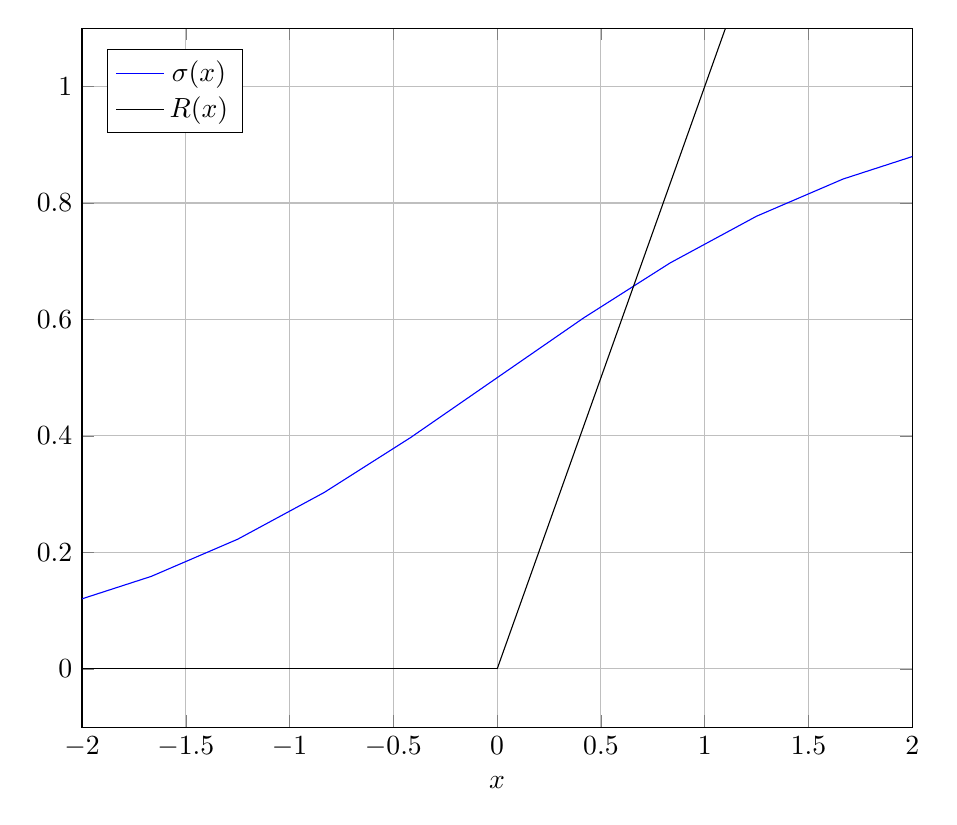
\begin{tikzpicture}
     \begin{axis} [
       grid=both,minor tick num=0,
      legend pos=north west,
      legend/.style={font=\small},
      xmin=-2,xmax=2,
      ymin=-.1,ymax=1.1,
      xlabel=$x$,
      width=\linewidth,
     ]
     \addplot[mark=none,blue] {1/(1+exp(-x))};
     \addlegendentry{$\sigma(x)$}
     % \only<2>{
      \addplot[mark=none,domain=-2:0] {0};
      \addplot[mark=none,domain=0:2] {x};
      \addlegendentry{$R(x)$}
     %}
    \end{axis}
   \end{tikzpicture}
  \end{column}
  \begin{column}{\linewidth/5*2}
   \begin{itemize}
    \item sigmoid
     \[
      \sigma(x) = \frac{1}{1+\mathrm{e}^{-x}}
     \]
    \item<2> ReLU (scaled)
     \[
      R(x) = \begin{cases}
       0 & x \leq 0 \\
       x & x > 0\\
      \end{cases}
     \]
   \end{itemize}
  \end{column}
 \end{columns}
\end{frame}

%% input to MLP

% \expandafter\newcommand\csname inVal0\endcsname{.5}
% \expandafter\newcommand\csname inVal1\endcsname{.9}
% \expandafter\newcommand\csname inVal2\endcsname{-.3}
% \expandafter\newcommand\csname hid0Weight0\endcsname{1}
% \expandafter\newcommand\csname hid0Weight1\endcsname{-2}
% \expandafter\newcommand\csname hid0Weight2\endcsname{2}
% \expandafter\newcommand\csname hid1Weight0\endcsname{2}
% \expandafter\newcommand\csname hid1Weight1\endcsname{1}
% \expandafter\newcommand\csname hid1Weight2\endcsname{4}
% \expandafter\newcommand\csname hid2Weight0\endcsname{1}
% \expandafter\newcommand\csname hid2Weight1\endcsname{-1}
% \expandafter\newcommand\csname hid2Weight2\endcsname{0}

% \expandafter\newcommand\csname out0Weight0\endcsname{-3}
% \expandafter\newcommand\csname out0Weight1\endcsname{1}
% \expandafter\newcommand\csname out0Weight2\endcsname{-3}
% \expandafter\newcommand\csname out1Weight0\endcsname{0}
% \expandafter\newcommand\csname out1Weight1\endcsname{1}
% \expandafter\newcommand\csname out1Weight2\endcsname{2}
% \renewcommand{\inText}[1]{
%  $\num{\csname inVal#1\endcsname}$
% }
% \expandafter\newcommand\csname hidVal0\endcsname{.13}
% \expandafter\newcommand\csname hidVal1\endcsname{.96}
% \expandafter\newcommand\csname hidVal2\endcsname{.40}
% \renewcommand{\hidText}[1]{
%  \only<1-2>{$H_{#1}$}%
%  \only<3->{%
%   $\num{\csname hidVal#1\endcsname}$
%  }%
% }
% \expandafter\newcommand\csname outVal0\endcsname{.35}
% \expandafter\newcommand\csname outVal1\endcsname{.85}
% \renewcommand{\outText}[1]{
%  \only<1-4>{$O_{#1}$}%
%  \only<5->{%
%   $\num{\csname outVal#1\endcsname}$
%  }%
% }
% \renewcommand{\synapseIHText}[2]{%
%  \only<2->{\ifthenelse{\equal{#1}{1}}
%  {}{\num{\csname hid#2Weight#1\endcsname}}}%
% }
% \renewcommand{\synapseHOText}[2]{%
%  \only<4->{\num{\csname out#2Weight#1\endcsname}}%
% }

% \begin{frame}
%  \frametitle{Artificial Neural Networks II}
%  \begin{center}
%   \tikzANN{}
%  \end{center}
% \end{frame}

   \begin{frame}
     \frametitle{Further Reading}

     \vfill
     \begin{itemize}
     \item Excellent overview of optimisation algorithms \href{https://ruder.io/optimizing-gradient-descent/}{ruder.io/optimizing-gradient-descent}
     \item a classic resource getting introduced to gradient descent \href{https://cs231n.github.io/optimization-1/}{Stanford CS231n}
     \end{itemize}
     \vfill
   \end{frame}

\end{document}
